\documentclass[11pt]{article}
\usepackage[top = 1.75cm]{geometry}                
\usepackage{amsmath}
\geometry{letterpaper}              
\usepackage{xfrac}\usepackage[parfill]{parskip}    % Activated to begin paragraphs with an empty line rather than an indent
\usepackage{graphicx}
\usepackage{amssymb}
\usepackage{epstopdf}
\interfootnotelinepenalty=10000
\DeclareGraphicsRule{.tif}{png}{.png}{`convert #1 `dirname #1`/`basename #1 .tif`.png}

\title{Portfolio Optimization and Risk Aversion in MATLAB}
\author{Adam Rosenbloom, Sean Kilachand, and Stuart Davis}

\newcommand*\justify{
	\hyphenchar\font=`\-
}

\begin{document}
\maketitle

\section*{Foreword}

This project determines an optimal portfolio given an individuals age and annual income.  The optimal portfolio will be comprised of five industry portfolios, as well as a risk-free asset.  This document has been written for investment professionals, but knowing that it would reach a broader audience, many statistical and financial concepts are elaborated on in the footnotes.  All returns and standard deviations are expressed as annual percentages.  Throughout this document, we will characterize probability distributions of rates of returns in terms of their expected or mean returns, \textit{E(r)}, and their standard deviations, $\sigma$.

We begin our analysis by characterizing the industry portfolios, and eventually determine an optimal risky portfolio through mean-variance optimization.  Once the optimal risky portfolio has been determined, the next fundamental allocation choice is how much of the complete portfolio to place in the risk-free asset versus the risky asset.  The optimal complete portfolio is dependent on an individual's risk aversion; to calculate this value, we use a fuzzy logic system that determines a risk aversion level based on annual income and age.  Ultimately, these calculations are used to recommend an investment portfolio.

\section{The Data and Statistics}

The data was taken from the database of Kenneth R. French's website.\footnote{French and co-author Eugene F. Fama are well known for their research into the Fama-French three-factor model.} The returns were given as monthly data beginning in July 1926 and continuing through December 2010.  All the monthly statistics have been annualized (doing so allows us to work in conventional annual units), but by initially using monthly data we have a larger sample size, and therefore better estimates of return, variance, and standard deviation.

The five industry portfolios are constructed by assigning each NYSE, AMEX, and NASDAQ stock to an appropriate industry portfolio.\footnote{The New York Stock Exchange (NYSE), American Stock Exchange (AMEX), and NASDAQ are all American stock exchanges located in New York City, New York.}  The assignment of a stock to an industry portfolio is based on its four-digit SIC code.\footnote{The Standard Industrial Classification (abbreviated SIC) is a US government system for classifying industries by a four-digit code.  The SIC codes are listed in a business's filings in order to indicate the industry to which the company belongs.  For example code 2024 corresponds to Ice Cream \& Frozen Desserts.}

French defines the five industry portfolios as:

\begin{enumerate}
	\item{Cnsmr: Consumer durables, non-durables, wholesale, retail, and some services (laundries, repair shops)}
	\item{Manuf: Manufacturing, energy, and utilities}
	\item{HiTec: Business equipment, telephone and television transmission, computer programming, data processing, information retrieval services, computer rental and leasing, computer facilities management, computer related services, R\&D labs}
	\item{Hlth: Healthcare, medical equipment, and pharmaceutical drugs}
	\item{Other: Mines, construction, building materials, transportation, hotels, business services, entertainment, and finance}
\end{enumerate}

The expected rate of return is the arithmetic average of the rates of return over the period.  Each observation (monthly return) was treated as an equally likely ``scenario''.  The standard deviation of the rate of return ($\sigma$) is a measure of risk.\footnote{It is defined as the square root of the variance, which in turn is the expected value of the squared deviations from the expected return. The higher the volatility in outcomes, the higher will be the average value of these squared deviations. Therefore, variance and standard deviation measure the uncertainty of outcomes.}  Below are the annualized expected returns and standard deviations for the five portfolios.  After annualizing the data, these moments can be found using the standard MATLAB functions \texttt{mean} and \texttt{std}.
\begin{center}
	\begin{tabular}{| l | c | c | c | c | c |} \hline
			& Cnsmr & Manuf & HiTec & Hlth & Other \\ \hline
			Mean & 11.883\% & 11.779\% & 11.147\% & 12.826\% & 10.790\%\\
			Standard Dev. & 18.686\% & 19.347\% & 19.726\% & 19.934\% & 22.720\%\\ \hline
	\end{tabular}
\end{center}
We also need two other important measures for the analysis: covariance and correlation.\footnote{The covariance is a measure of linear association between two variables. Positive values indicate a positive relationship, and negative values indicate a negative relationship. Similarly, the correlation coefficient is a measure of linear association between two variables that takes on values between -1 and +1. Values near one indicate a strong positive linear relationship, values near negative one indicate a strong negative relationship, and values close to zero indicate the lack of a linear relationship. The two measurements reflect essentially the same information, but the correlation coefficient is easier to interpret.}  Covariance and coefficient of correlation can be computed in MATLAB by calling the \texttt{cov} and \texttt{corrcoef} functions respectively.  Below is the coefficient of correlation matrix for the five industry portfolios:
\begin{center}
	\begin{tabular}{| l | c | c | c | c | c |} \hline
		& Cnsmr & Manuf & HiTec & Hlth & Other \\ \hline
		Cnsmr & 1 & 0.8749 & 0.8103 & 0.7784 & 0.8777 \\
		Manuf & 0.8749 & 1 & 0.8086 & 0.7491 & 0.8927 \\
		HiTec & 0.8103 & 0.8086 & 1 & 0.7099 & 0.7949 \\ 
		Hlth &  0.7784 & 0.7491 & 0.7099 & 1 & 0.7405 \\
		Other & 0.8777 & 0.8927 & 0.7949 & 0.7405 & 1 \\ \hline
	\end{tabular}
\end{center}
Obviously each portfolio is perfectly correlated to itself.  The lower the correlation, the better the two assets hedge (reduce) market risk.

\section{The Portfolio Opportunity Set}
We turn our attention now to constructing the risky portfolio.  We started by examining a large range of possible risky portfolios.  We generated five thousand random risky portfolios, each with different percentages of capital invested in the five industry portfolios.  These different combinations of assets display different combinations of return and risk possible by investing in a portfolio of the five industry portfolios.  These points, plotted below in black, are called the portfolio opportunity set because they provide many of the combinations of portfolio expected returns and standard deviations that can be constructed from these five assets.  The individual assets are also plotted below as red asterisks.  Notice that the opportunity set is ``pulled'' to the northwest because of the benefits of diversification.\footnote{In finance, diversification refers to reducing risk by investing in a variety of assets.  If the asset values are not perfectly correlated, a diversified portfolio will have less risk than the weighted average risk of constituent assets, and often less risk than the least risky of its constituents.}  The \texttt{portrand} function in the Financial Toolbox generates a portfolio opportunity set.  Portfolios are selected at random from a set of portfolios such that portfolio weights are non-negative and sum to 1.
\begin{figure}[h]
	\begin{center}
		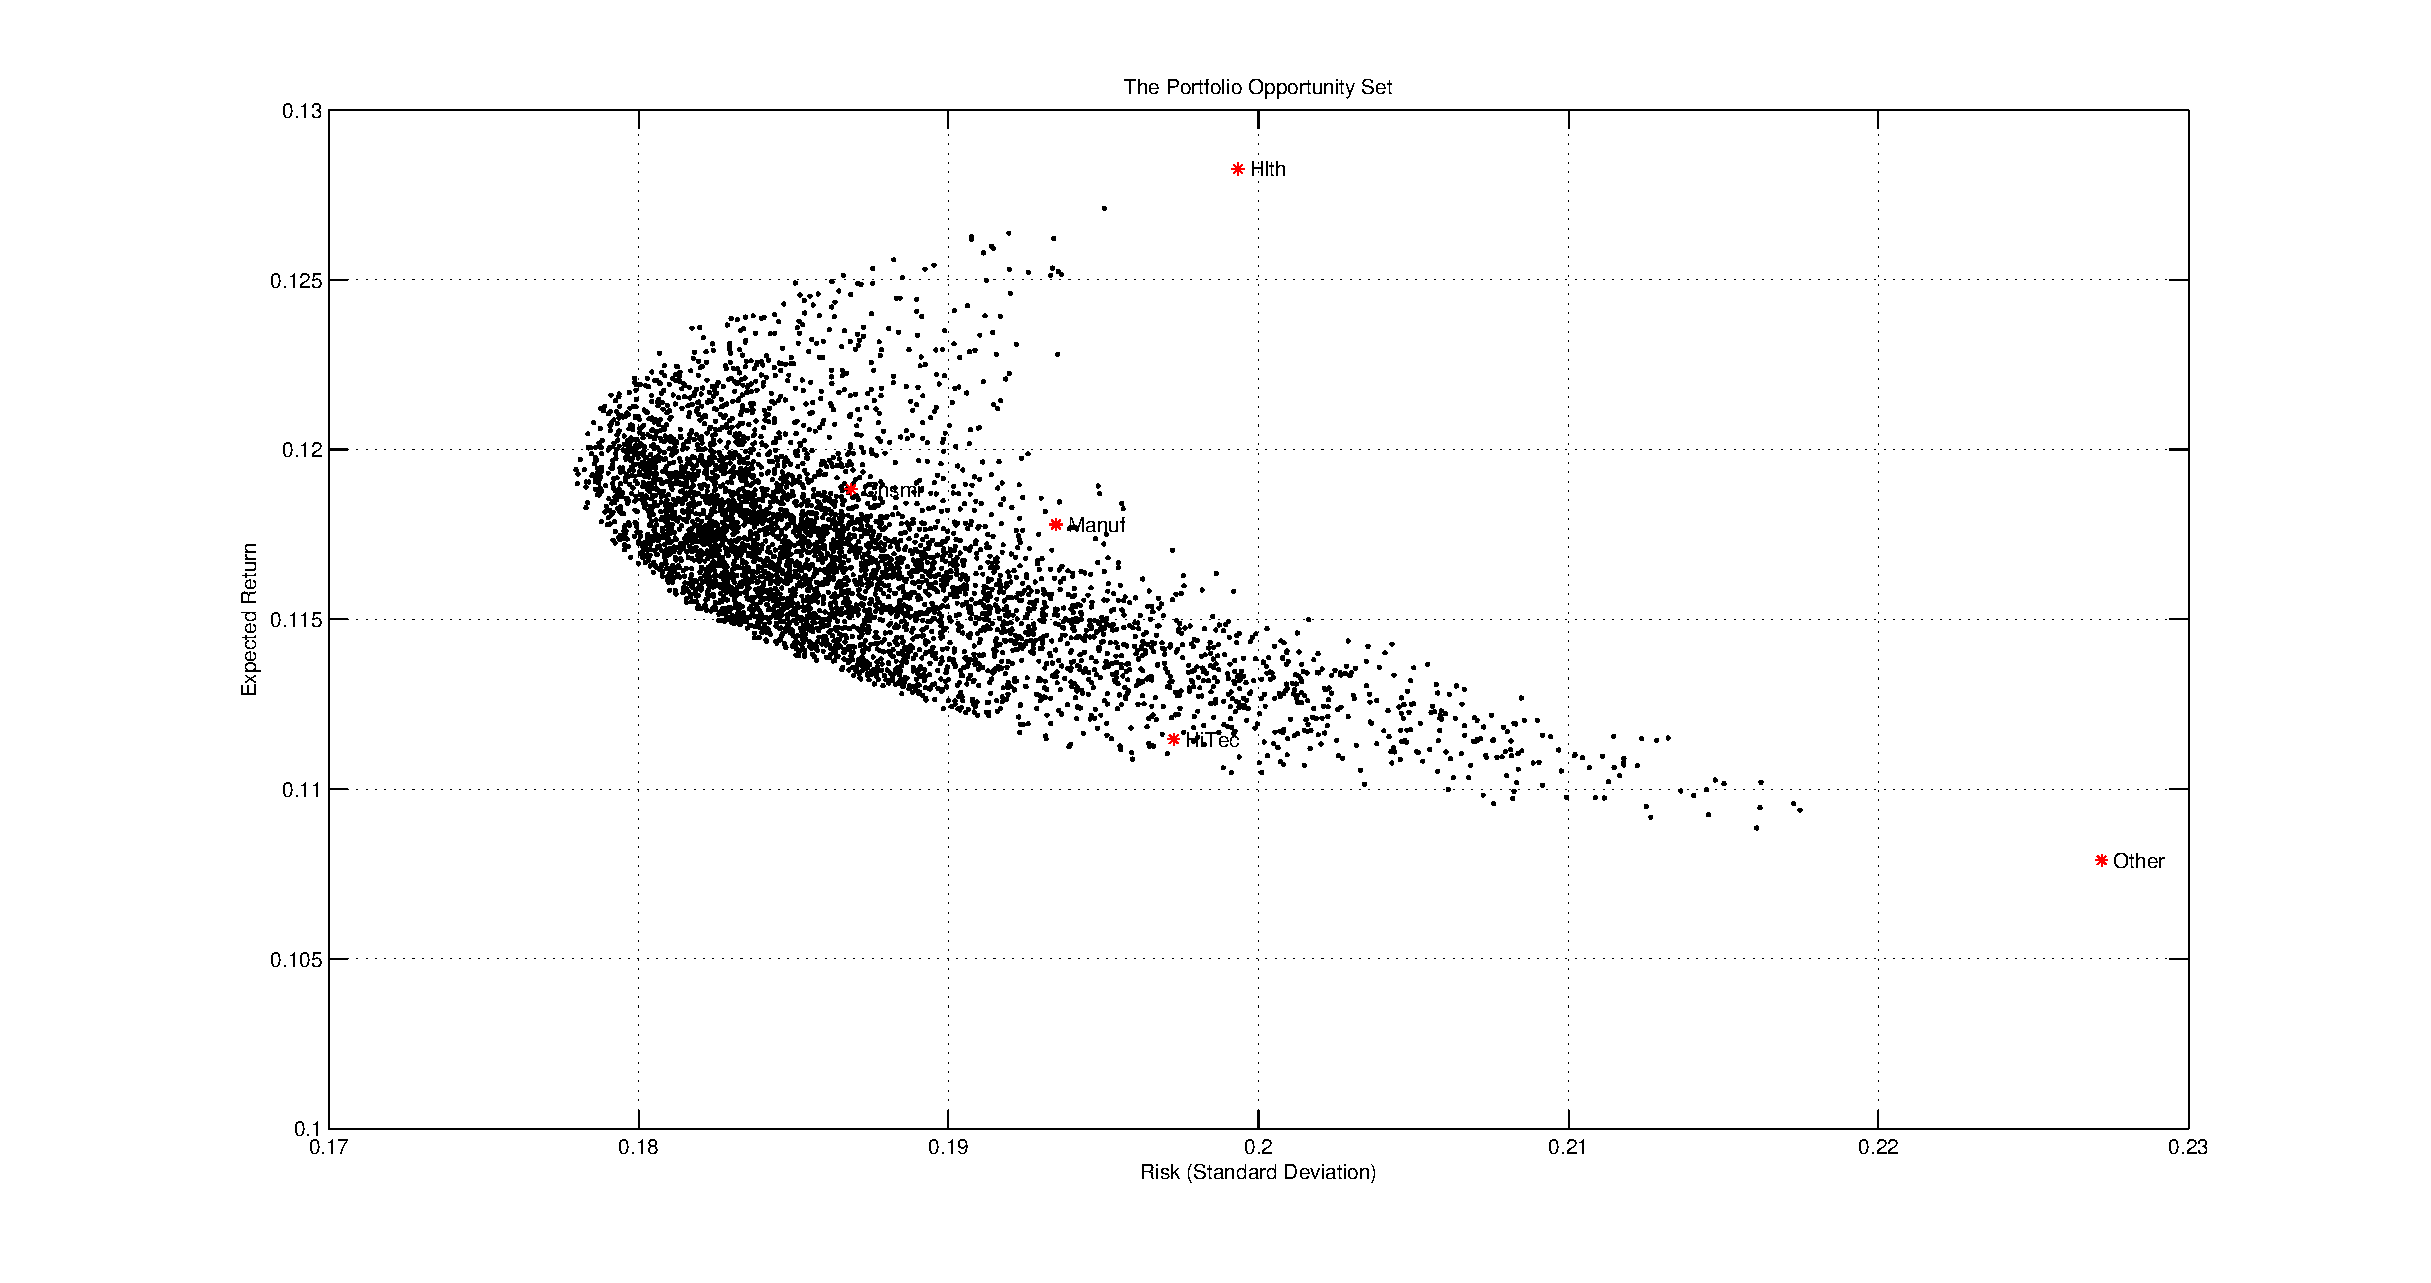
\includegraphics[scale = .39]{POS.eps}
		\caption{The portfolio opportunity set based on the the five industry portfolios.}
	\end{center}
\end{figure}
\section{The Efficient Frontier}
One of the most obvious features of the portfolio opportunity set is that it contains some portfolios that are inferior to others.  That is, some portfolios have more risk (higher standard deviation) for less reward (expected return).\footnote{This is the mean-variance criterion: portfolio A dominates B if the expected return of A is greater than or equal to the expected return of B and the standard deviation of A is less than or equal to B and at least one inequality is strict (rules out the equality).}  For example, any portfolio that lies to the northwest of the HiTec portfolio is superior to it, and any portfolio that lies to the southeast is inferior.

If these inferior portfolios are eliminated, then only the efficient frontier of risky assets remains.  The efficient frontier displays all the portfolios that provide the best risk-return combinations, and thus are candidates for the optimal risky portfolio.  It is a graph of the lowest possible risk that can be attained for a given portfolio's expected return.  The leftmost point represents the global minimum-variance risky portfolio.  The Financial Toolbox function \texttt{[PortRisk, PortReturn, PortWts] = frontcon(ExpReturn, ExpCovariance, NumPorts)} returns the efficient frontier.  If you invoke \texttt{frontcon} without output arguments, it generates a plot of the efficient frontier.  The efficient frontier generated in that way is shown below.

\begin{figure}[h]
	\begin{center}
		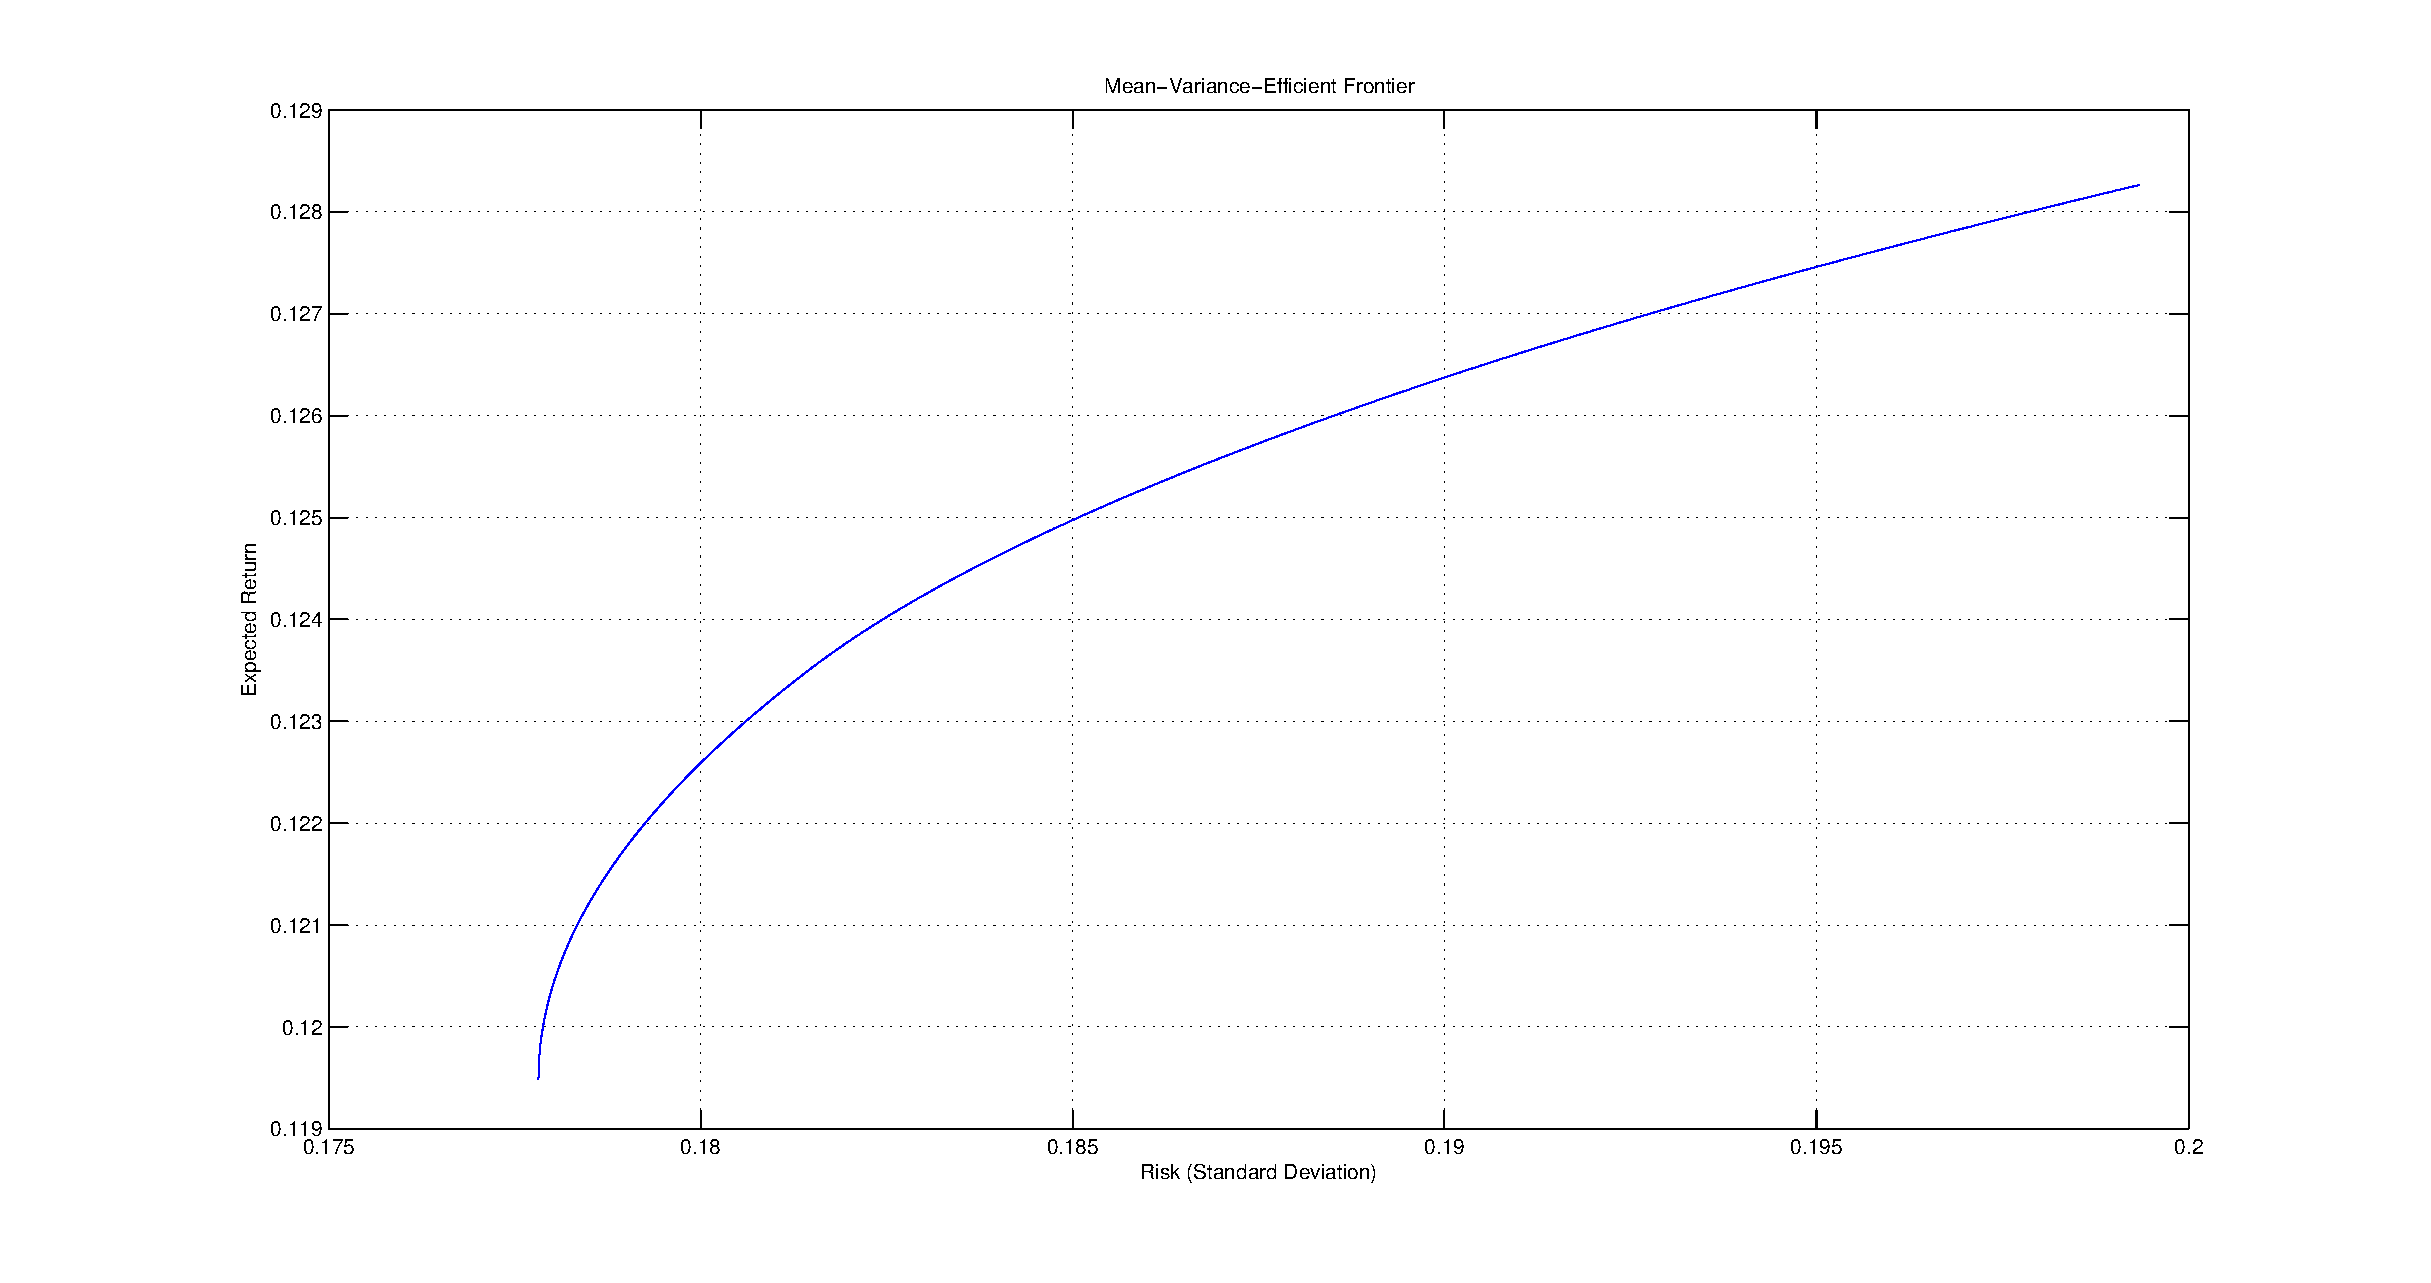
\includegraphics[scale = .39]{EfficientFrontier.eps}
		\caption{The efficient frontier based on the five industry portfolios.  The leftmost point is the global minimum-variance portfolio.}
	\end{center}
\end{figure}

\section{The Optimal Risky Portfolio}
To establish the optimal risky portfolio, we maximized the reward-to-volatility (Sharpe ratio).\footnote{The Sharpe ratio is a return over risk ratio.  High values entail more return for less risk. Not taking into account individual risk preferences, the higher the Sharpe ratio, the more desirable the asset.}  It is a measure of the excess return over the risk-free rate (or risk premium) per unit of risk for a security.  In mathematical terms, 
	\[S = \frac{E\left(R\right) - r_f}{\sigma}\]
The aim is to find the weights in each asset that result in the highest Sharpe ratio.  Thus, the objective function is the Sharpe ratio, subject to the constraint that the portfolio weights must sum to 100\%.  This problem can be solved using the standard tools of calculus, and the Financial Toolbox provides the \texttt{portalloc} function to obtain the solution, shown below.  We will elaborate on this function later in the text.

\begin{center}
	\begin{tabular}{| c | c | c | c | c | c | c |} \hline
		$w_\textrm{\tiny{Cnsmr}}$ & $w_\textrm{\tiny{Manuf}}$ & $w_\textrm{\tiny{HiTec}}$ & $w_\textrm{\tiny{Hlth}}$ & $w_\textrm{\tiny{Other}}$ &\small{Annual \textit{E(r)}} & \small{Standard Deviation} \\ \hline
		34.239\% & 14.651\% & 2.645\% & 48.465\% & 0.000\% & 12.306\% & 18.070\%\\ \hline
	\end{tabular}
\end{center}

\section{The Capital Allocation Line}
Since we have now determined the composition of the risky portfolio, now the concern is with the proportion of the investment budget to be allocated to the risky portfolio.  The remaining proportion is to be invested in the risk-free asset.  The rate of return on the risk-free asset is denoted as $r_f$, and in this analysis, the risk-free rate is assumed at 1\%.\footnote{It is common practice to view Treasury bills as ``the'' risk-free asset.  Their short-term nature makes their values insensitive to interest rate fluctuations, and there is virtually zero default risk.  According to Dimson, Marsh \& Staunton, the mean real interest rate of US treasury bills during the 20$^{th}$ century was .9\%.}

The expected return of the complete portfolio as a function of its standard deviation is a straight line, with intercept $r_f$ and the Sharpe ratio as slope.  This line, called the capital allocation line (CAL), represents the set of feasible expected return and standard deviation pairs of all portfolios resulting from different amounts of capital invested in the risky portfolio.  The CAL is shown below in pink, superimposed on the efficient frontier.  Notice that the CAL is tangent with the efficient frontier at the optimal portfolio.  This demonstrates that the CAL has the highest feasible reward-to-volatility ratio.  The optimal risky portfolio is shown below as a black asterisk.

\begin{figure}[h]
	\begin{center}
		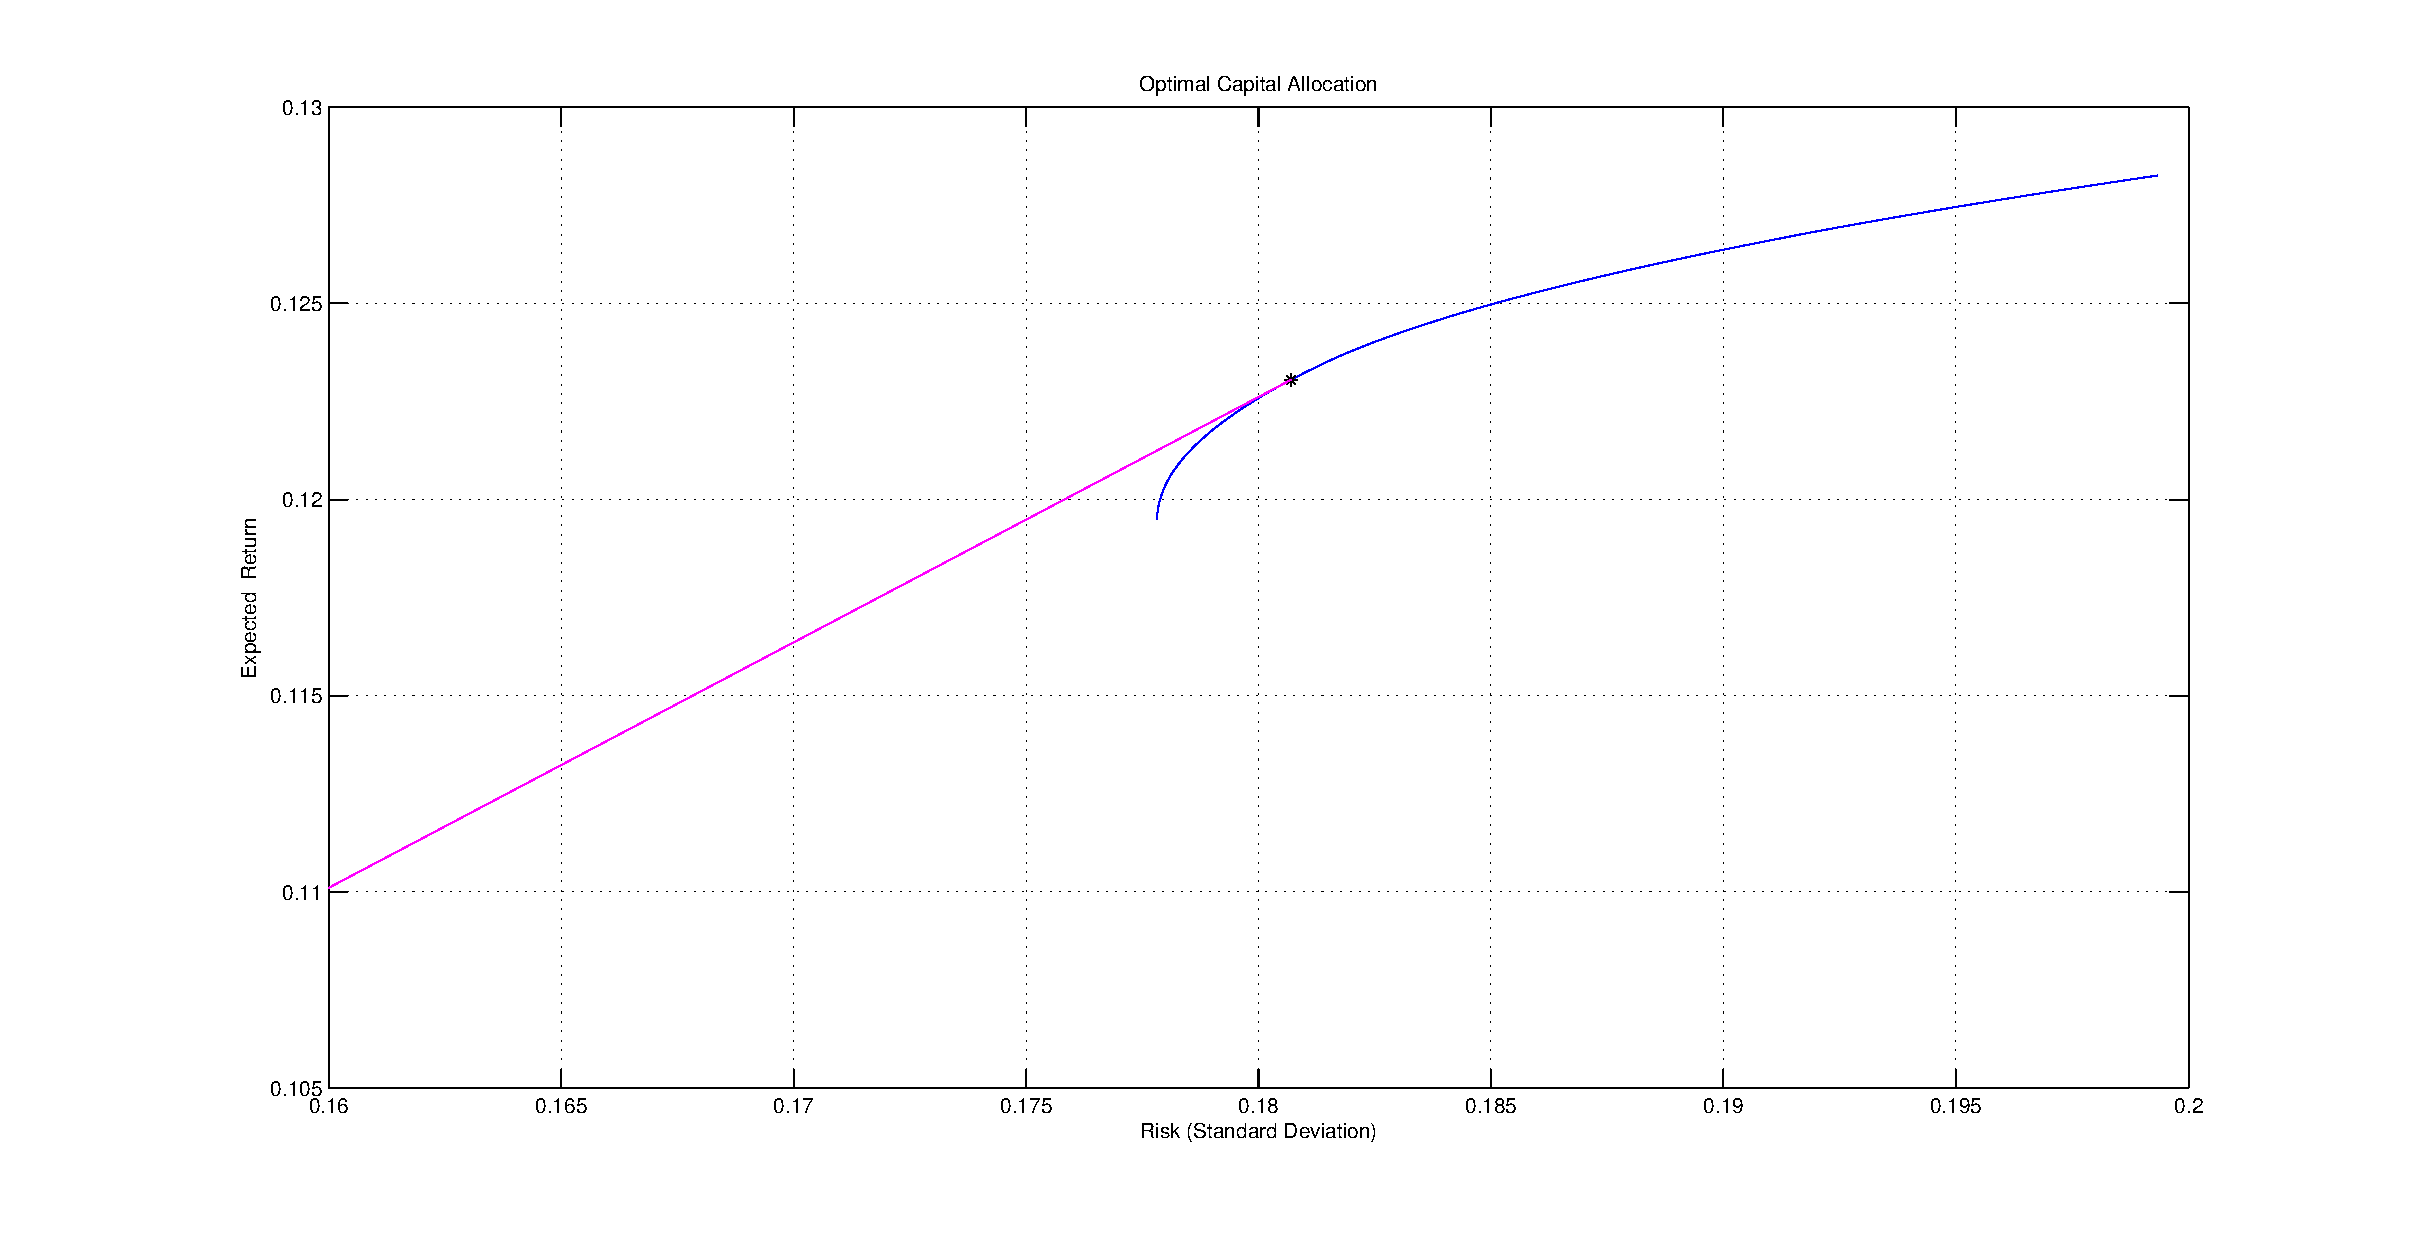
\includegraphics[scale = .39]{OptimalCapAlloc.eps}
		\caption{The efficient frontier and the capital allocation line.}
	\end{center}
\end{figure}

\section{Risk Aversion and Fuzzy Logic}
Risky assets command a risk premium in the marketplace, which implies that most investors are risk averse.  Risk aversion is the reluctance of a person to accept a bargain with an uncertain payoff rather than another bargain with a more certain, but possibly lower, expected payoff. Investors who are risk averse reject investment portfolios that are fair games or worse. Loosely speaking, a risk-averse investor �penalizes� the expected rate of return of a risky portfolio by a certain percentage to account for the risk involved. The greater the risk, the larger the penalty. Risk-neutral investors (\textit{A} = 0) judge risky prospects solely by their expected rates of return.  To determine an individual's optimal complete portfolio, we must try to gauge his or her risk aversion level.
	
Fuzzy logic provides mathematical calculation using fluid values rather than boolean values.\footnote{Boolean values accept a value of either true (1) or false (0).}  Boolean values have only two values, where as fuzzy logic provides a value derived from comparing an set of input's values relative to each other. Fuzzy logic is useful for deriving continuous variables where the resulting truth value is dependent on the input's relative difference. Fuzzy logic uniquely translates a numerical value into a linguistic term representing the range containing the number.

In our implementation, an individual's risk aversion is determined depending on his/her income and age. Risk aversion, annual income and age have three possible terms. Risk aversion's term set is Low, Middle, and High. Annual income's term set is also Low, Medium, and High. The age term set is Young, Middle, and Old. These fuzzy numbers representing risk aversion, annual income, and age belong to the universal sets (respectively): 
	\begin{align*}
		A &= \left\{a \, | \, 0 \leq a \leq 10\right\}\\
		B &= \left\{b \times 10^3 \, | \, 0 \leq b \leq 1000\right\}\\
		C &= \left\{c \, | \, 0 \leq c \leq 120\right\}. 
	\end{align*}
The abstract value \textit{a} represents a psychological measure of risk aversion between 0 and 10. The real numbers \textit{b} and \textit{c} represent annual income in thousands of dollars and ages between 0 and 120 years. We used trapezoidal membership functions to describe the two inputs (annual income and age) and the output (risk aversion).

There are nine possible combinations of terms because each input has three values. Given in the format (Income, Age) = Risk Aversion, these nine combinations must correspond to one of three output (risk aversion) values.
\begin{align*}
	(Low, Young) &= Medium\\
	(Low, Middle) &= High\\
	(Low, Old) &= High\\
	(Middle, Young) &= Low\\
	(Middle, Middle) &= Medium\\
	(Middle, Old) &= High\\
	(High, Young) &= Low\\
	(High, Middle) &= Low\\
	(High, Old) &= Medium
\end{align*}
Based on these rules, we can estimate an individual's risk aversion given age (in years) and annual income (in thousands of dollars). The graphs below represent the membership functions for the two inputs and one output:

\begin{figure}[h]
	\begin{center}
		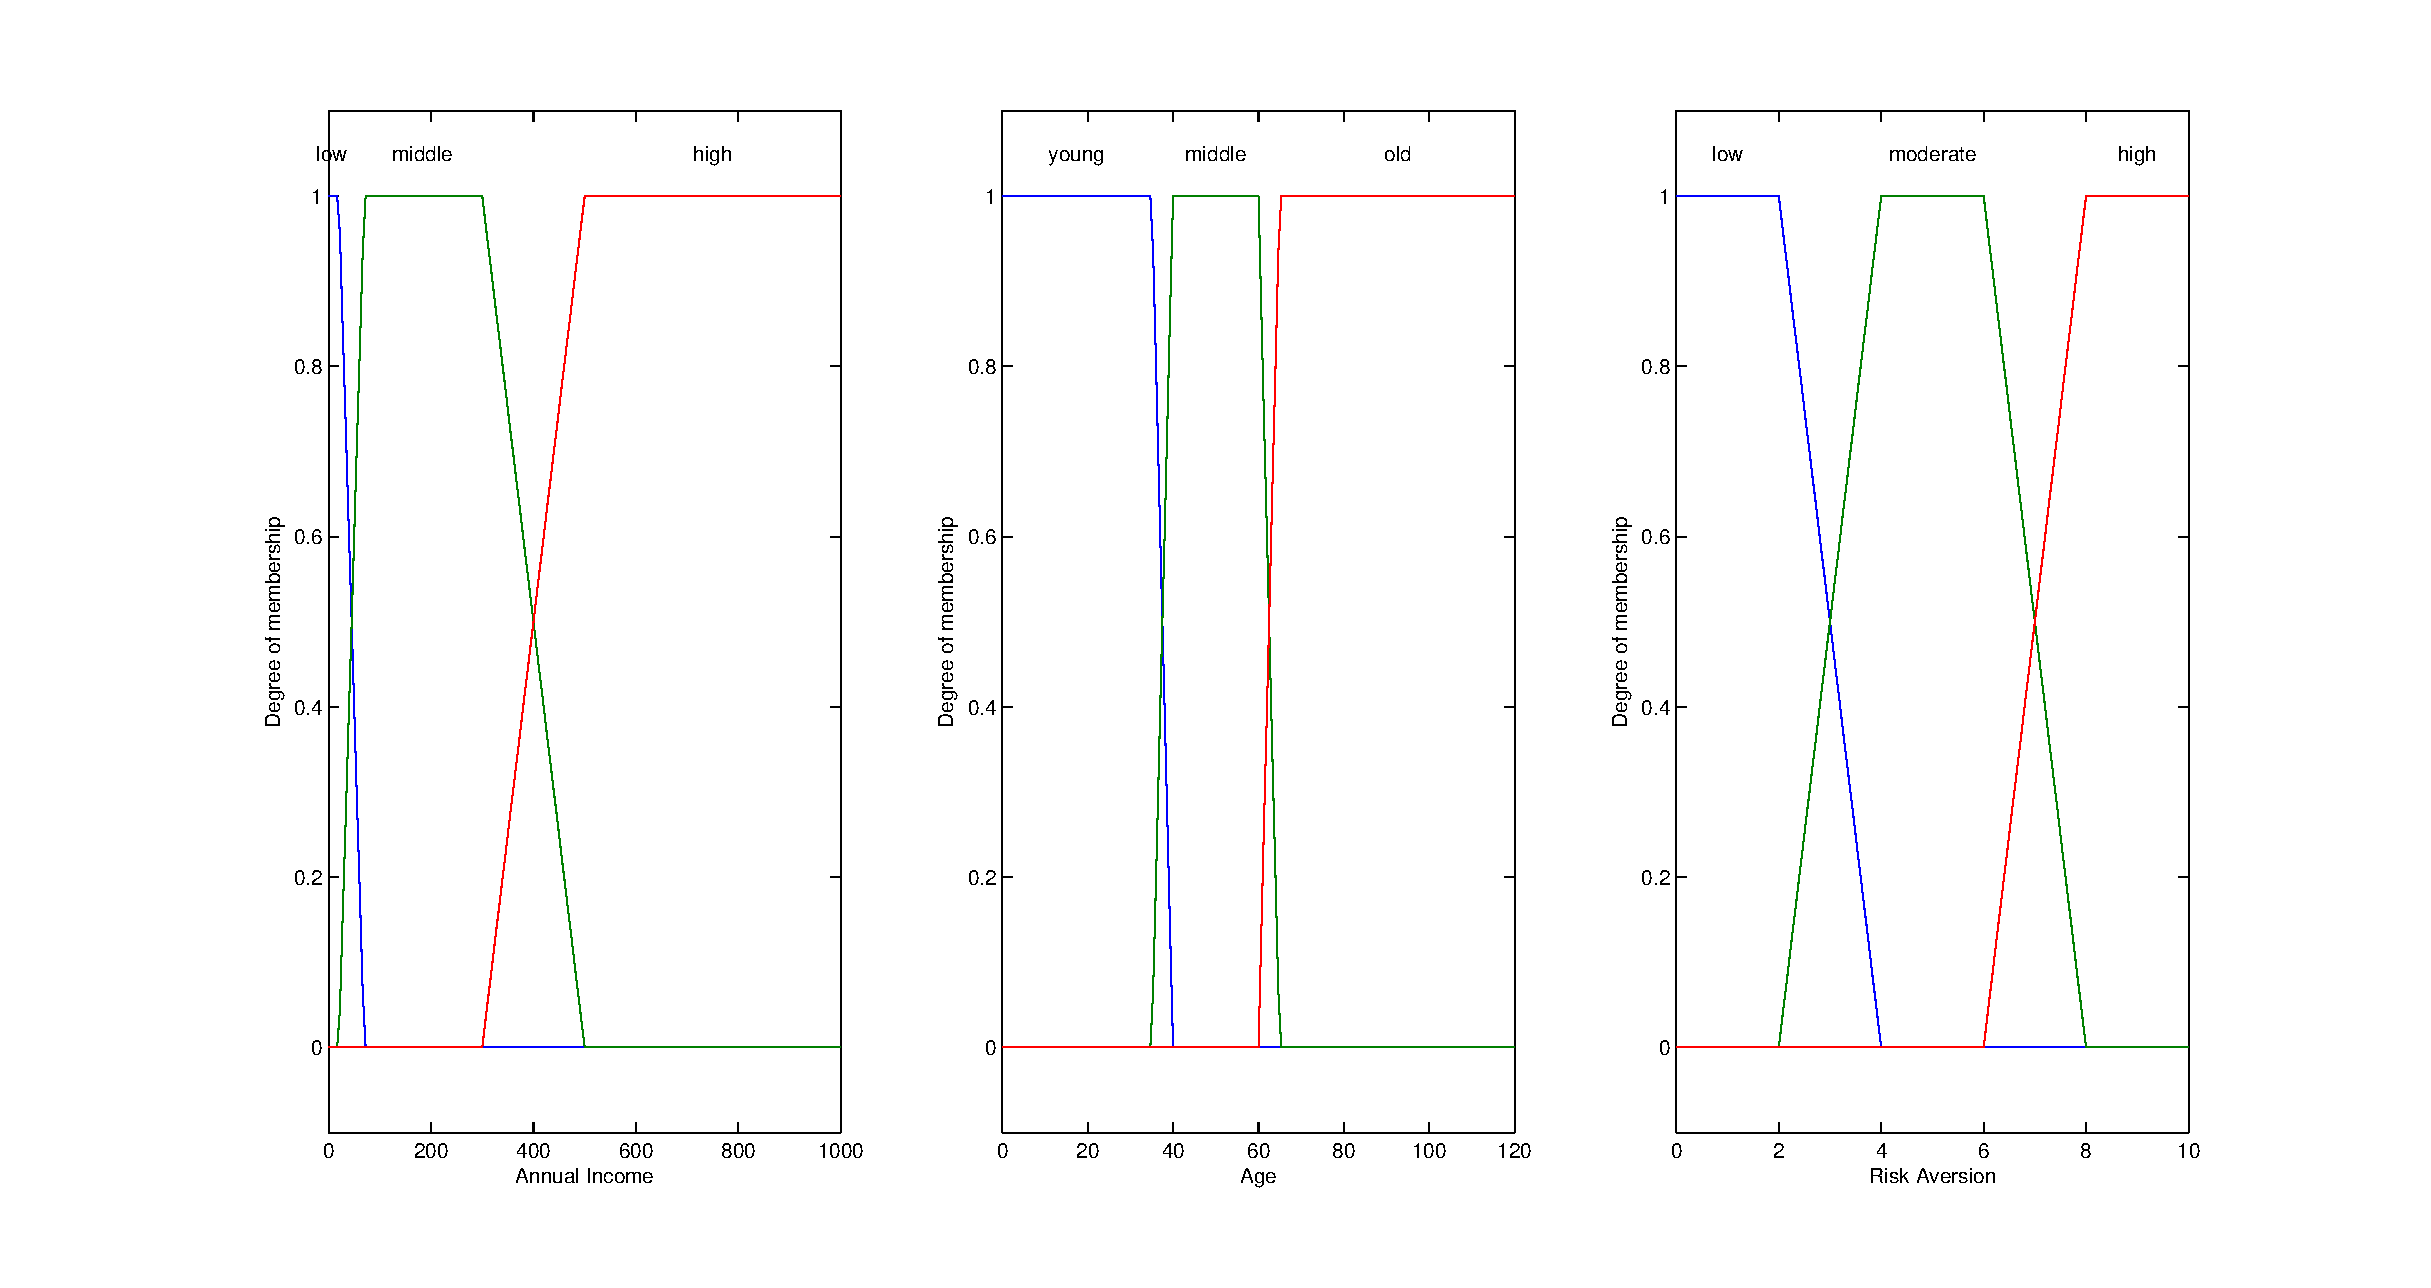
\includegraphics[scale = .39]{MembershipFunctions.eps}
		\caption{The membership functions for the fuzzy interface system used to determine risk aversion 			       based on income and age.}
	\end{center}
\end{figure}

The term describing each linguistic variable is determined using a trapezoidal function where the range of each term is demonstrated by the graph. For example, for annual income, the variable's term is calculated by finding which membership function the variable exists within (for example, an annual income of \$50,000 falls in the medium membership function).

The following plot represents the fuzzy logic system that solves the risk aversion problem:

\begin{figure}[h]
	\begin{center}
		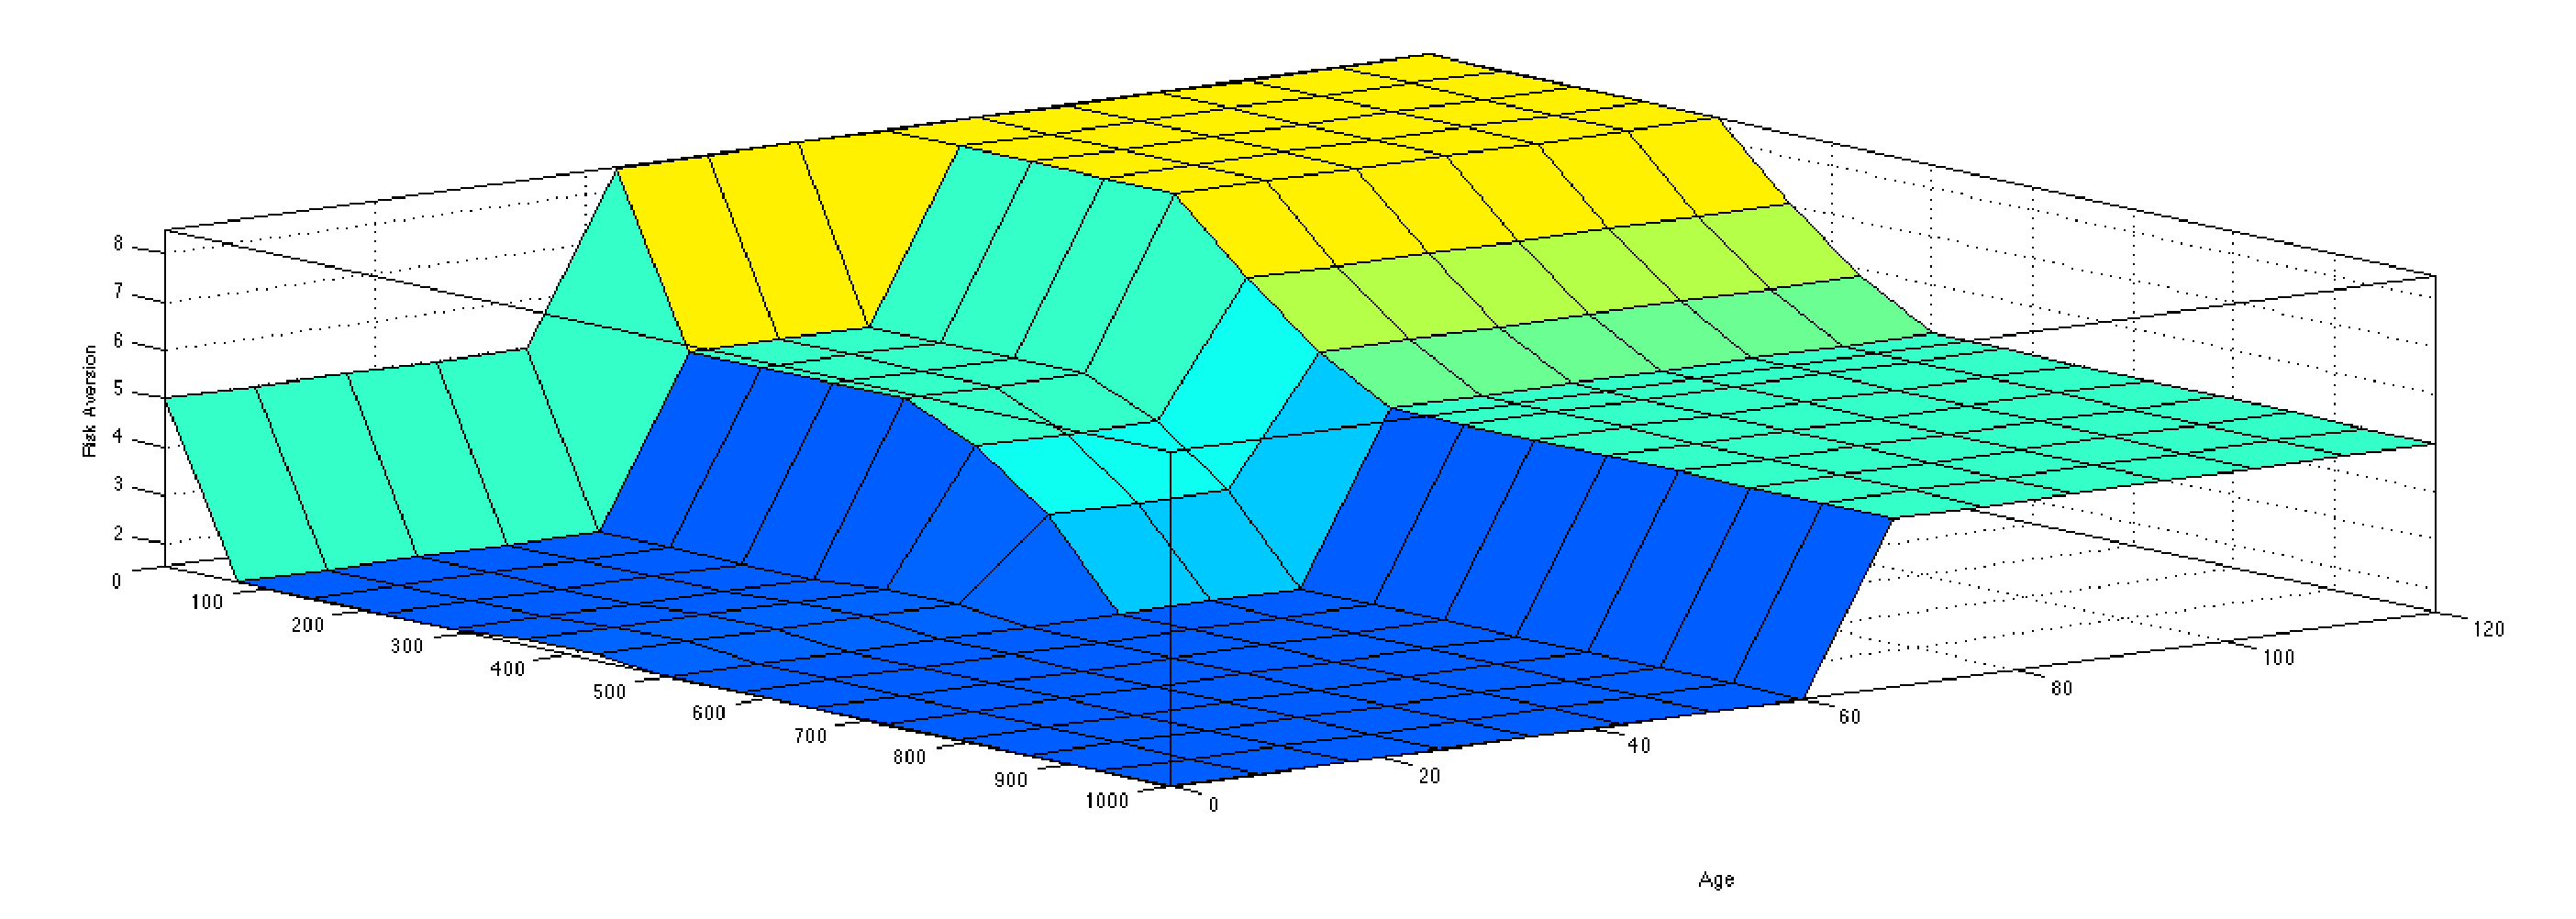
\includegraphics[scale = .3]{FisGraph.eps}
		\caption{The solution to the risk aversion problem solved by the fuzzy logic system.}
	\end{center}
\end{figure}

\section{Maximizing Utility}
Next, we can assign a utility, or welfare, score to competing investment portfolios based on the expected return and risk of those portfolios, and the individual investor's degree of risk aversion.  One reasonable function that has been employed by both financial theorists and the CFA Institute assigns a portfolio with expected return \textit{E(r)} and variance of returns $\sigma^2$ a utility score of $U=E(r) - \left(\sfrac{1}{2}\right)A\sigma^2$.  This is the default utility function in the Financial Toolbox.  Individual investor differences in risk aversion imply that, given an identical opportunity set, different investors will choose different positions in the risky asset.  To solve the utility maximization problem, we take the derivative of the utility function with respect to the percentage of funds invested in the risky portfolio, then set this expression equal to zero and solve for the weight of the risky portfolio.\footnote{The optimal position in the risky asset is inversely proportional to the level of risk aversion and directly proportional to the risk premium offered by the risky asset.}

Below, we have maximized the utilities for two investors with different risk aversion levels and determined the optimal allocations between the risky portfolio and the risk-free asset, in addition to the characteristics of the complete portfolio.  The results are summarized below:
\begin{center}
	\begin{tabular}{| l | c | c |} \hline
		& Aversion = 4 & Aversion = 8\\ \hline
		Percent of Capital Invested in the Risky Portfolio & 86.56\% & 42.280\%\\
		Percent of Capital Invested in T-Bills & 13.440\% & 56.720\%\\
		Expected Return of the Complete Portfolio & 10.786\% & 5.893\%\\
		Standard Deviation of the Complete Portfolio & 15.641\% & 7.821\%\\ \hline
	\end{tabular}
\end{center}

\begin{figure}[h]
	\begin{center}
		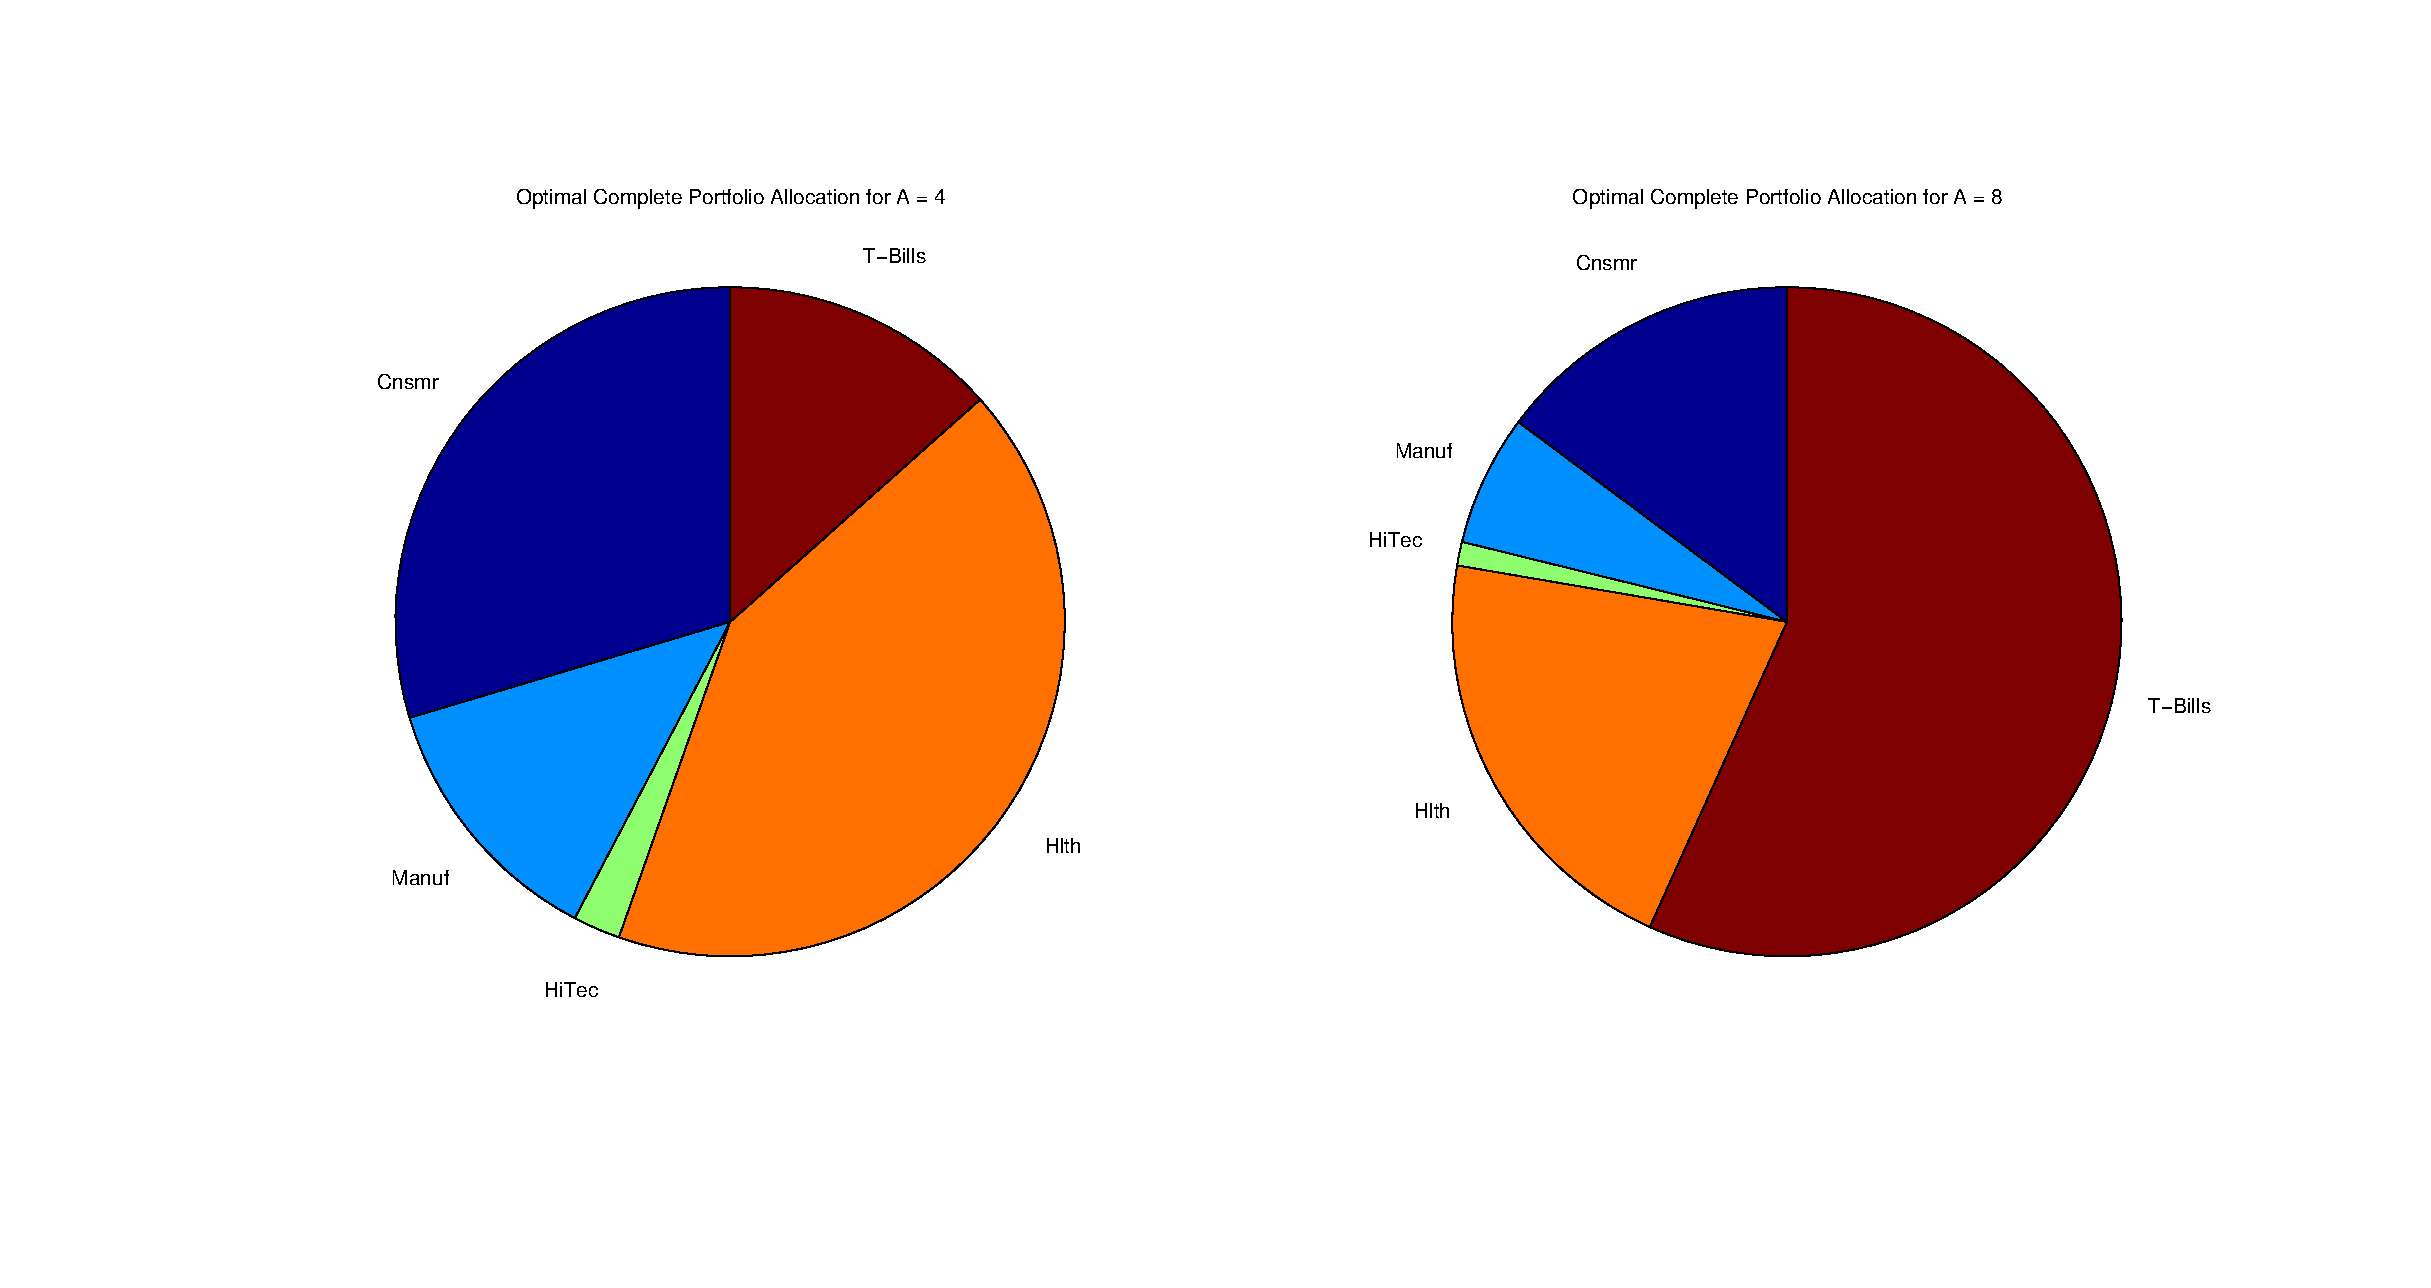
\includegraphics[scale = .39]{AversionCompleteAlloc.eps}
	\end{center}
\end{figure}

The most readily apparent fact is that more risk averse investors hold less of the risky portfolio.  Therefore, their portfolios will have lower expected return and also lower standard deviation than less risk averse investors.

These results were obtained by utilizing the \texttt{portalloc} function. \texttt{\justify[RiskyRisk, RiskyReturn, RiskyWts, RiskyFraction, OverallRisk, OverallReturn] = portalloc (PortRisk, PortReturn, PortWts, RisklessRate, BorrowRate, RiskAversion)} computes the optimal risky portfolio, and the optimal allocation of funds between the risky portfolio and the risk-free asset.  When \texttt{portalloc} is invoked without output arguments, it generates a plot of the optimal capital allocation.

In modern portfolio theory, the optimal risky portfolio is usually the same for all investors, since it is based on mean-variance optimization.  However, the \texttt{portalloc} function has a sophisticated property: if an investor has low enough risk aversion that 100\% of all capital will be invested in the risky portfolio, it will redetermine the allocations of the risky portfolio to maximize utility based on the aforementioned utility function.

\section{Concluding Thoughts}
Finally, we have arrived at two complete portfolios.  To summarize: we first established the optimal risky portfolio by using mean-variance optimization.  Then, we determined risk aversion levels by implementing a fuzzy logic system that had rules based on age and annual income.  Finally, we used that risk aversion level to determine the ideal allocation of funds between the optimal risky portfolio and the risk-free asset by maximizing utility.

This theory is formally called modern portfolio theory.  It was developed in the 1950s by Harry Markowitz and was considered an important advance in the mathematical modeling of finance.  It is widely used in practice in the financial industry, and Markowitz won a Nobel Memorial Prize in Economic Sciences for the theory.

\section{MATLAB Exercises}
	
	This comprehensive exercise has been included to help you internalize the fundamental concepts and vocabulary you have seen throughout this document.  It will walk you through an example of constructing a complete optimal portfolio from start to finish much like the process detailed above.  As you are working through this example, you are encouraged to look through our code to help your understanding.
	
	\subsection{Expected Return, Standard Deviation, and Covariance}
	In Section 1, we defined important statistical measures used in portfolio theory.  To refresh, expected return is the arithmetic average of the rates of return of a period, risk was defined as the standard deviation of the rate of return, and covariance was defined as a measure of linear association between two variables.  Given the following annual returns for three securities, securities \textit{a, b, c,} and \textit{d}, use the built-in MATLAB functions to:
	\begin{enumerate}
		\item{Compute \textit{E(R)}, the expected return of the three securities}
		\item{Compute $\sigma$, the risk of the securities}
		\item{Compute the covariance matrix of securities \textit{a, b, c} and \textit{d}}
	\end{enumerate}
	\begin{center}
		\begin{tabular}{| l | c | c | c | c |} \hline
			& \textit{a} & \textit{b} & \textit{c}\ & \textit{d}\\ \hline
			Year 1 & 7.259\% & 10.129\% & 7.419\% & 6.093\%\\
			Year 2 & 16.886\% & 7.057\% & 14.927\% & 1.905\%\\
			Year 3 & 9.228\% & 5.311\% & 7.904\%& 3.187\%\\
			Year 4 & 12.179\% & 11.491\% & 4.984\% & 2.653\%\\
			Year 5 & 28.065\% & 15.554\% & 4.833\%& 14.643\%\\
			Year 6 & 1.678\% & 13.460\% & 5.526\%& 3.763\%\\ 
			Year 7 & 5.662\% & 3.706\% & 3.615\% & 5.968\%\\
			Year 8 & 19.837\% & 6.447\% & 4.819\% & 2.454\%\\
			Year 9 & 8.737\% & 5.189\% & 6.642\% & 6.856\%\\
			Year 10 & 18.244\% & 14.810\% & 3.827\% & 6.003\%\\ \hline
		\end{tabular}
	\end{center}
	
	\subsection{The Portfolio Opportunity Set}
	The portfolio opportunity set is discussed in detail in Section 2.  Recall the definition: given a set of assets, the set of all portfolios that can be constructed at different levels of risk and expected return.  Using the built-in MATLAB function, plot the portfolio opportunity set for securities \textit{a, b, c} and \textit{d} (use 5,000 portfolios).  Also, plot the securities \textit{a, b, c} and \textit{d} on the graph of the portfolio opportunity set.  Based on your graph of the portfolio opportunity set, which security is considered the dominated security? (hint: see footnote 7)
	
	\subsection{The Efficient Frontier}
	The efficient frontier is discussed in detail in Section 3.  To refresh, a portfolio is referred to as ``efficient'' if it has the best possible expected level of return for its level of risk (usually proxied by the standard deviation of the portfolio's return).  Using the built-in MATLAB function, generate a plot of the efficient frontier of securities \textit{a, b, c} and \textit{d}.
	
	\subsection{Risk Aversion}
	Section 6 describes in detail a fuzzy logic system that will output risk aversion based on inputs annual income and age.  For advanced programmers, try to implement this system using the Fuzzy Logic toolbox in MATLAB.  For less advanced programmers, use ours.  Enter \texttt{fis = buildFIS()} in the MATLAB command line.  This will construct the fuzzy interface system and store it in variable \texttt{fis}.
	
	Now, use the fuzzy logic system to determine the risk aversion value for:
	\begin{enumerate}
		\item{a 20-year-old individual with annual income of \$45,000}
		\item{a 65-year-old individual with annual income of \$50,000}
	\end{enumerate}
		
	\subsection{Constructing the Optimal Complete Portfolio}
	Now, suppose you are the 65-year-old individual with annual income \$50,000 in the previous prompt who had a risk aversion value of 8.3077.  Using the built-in MATLAB tools, determine the composition of the optimal complete portfolio comprised of securities \textit{a, b, c} and \textit{d} and a risk-free asset with a 2\% rate of return ($r_f = .02$).  Do not allow for borrowing in this example.  What is the composition of the complete portfolio?  What is its expected return and standard deviation?
	
\section{Solutions to MATLAB Exercises}

	\subsection{Expected Return, Standard Deviation, and Covariance}

		\texttt{
		\begin{tabular}{ l l l l l}
			Returns = [& .07259 & .10129 & .07419 & .06093;\\
			& .16886 & .07057 & .14927 & .01905;\\
			& .09228 & .05311 & .07904 & .03187;\\
			& .12179 & .11491 & .04984 & .02653;\\
			& .28065 & .15554 & .04833 & .14643;\\
			& .01678 & .13460 & .05526 & .03763;\\ 
			& .05662 & .03706 & .03615 & .05968;\\
			& .19837 & .06447 & .04819 & .02454;\\
			& .08737 & .05189 & .06642 & .06856;\\
			& .18244 & .14810 & .03827 & .06003;];\\
		\end{tabular}
		}
\begin{verbatim}
  ExpReturns = mean(Returns,1)
  StdDev = std(Returns)
  Covariance = cov(Returns)
\end{verbatim}
	This code outputs:
	
\begin{verbatim}
  ExpReturns =
    0.1278    0.0932    0.0645    0.0535
  StdDev =
    0.0792    0.0434    0.0330    0.0372
  Covariance =
    0.0063    0.0013    0.0000    0.0014
    0.0013    0.0019   -0.0004    0.0007
    0.0000   -0.0004    0.0011   -0.0004
    0.0014    0.0007   -0.0004    0.0014
\end{verbatim}

\subsection{The Portfolio Opportunity Set}
\begin{verbatim}
  portrand(Returns, ExpReturns, 5000)
  hold on;
  plot(StdDev(1), ExpReturns(1), `sk') % Security a
  plot(StdDev(2), ExpReturns(2), `sk') % Security b
  plot(StdDev(3), ExpReturns(3), `sk') % Security c
  plot(StdDev(4), ExpReturns(4), `sk') % Security d
  hold off;
\end{verbatim}
which outputs the following graph: 
\begin{figure}[h]
	\begin{center}
		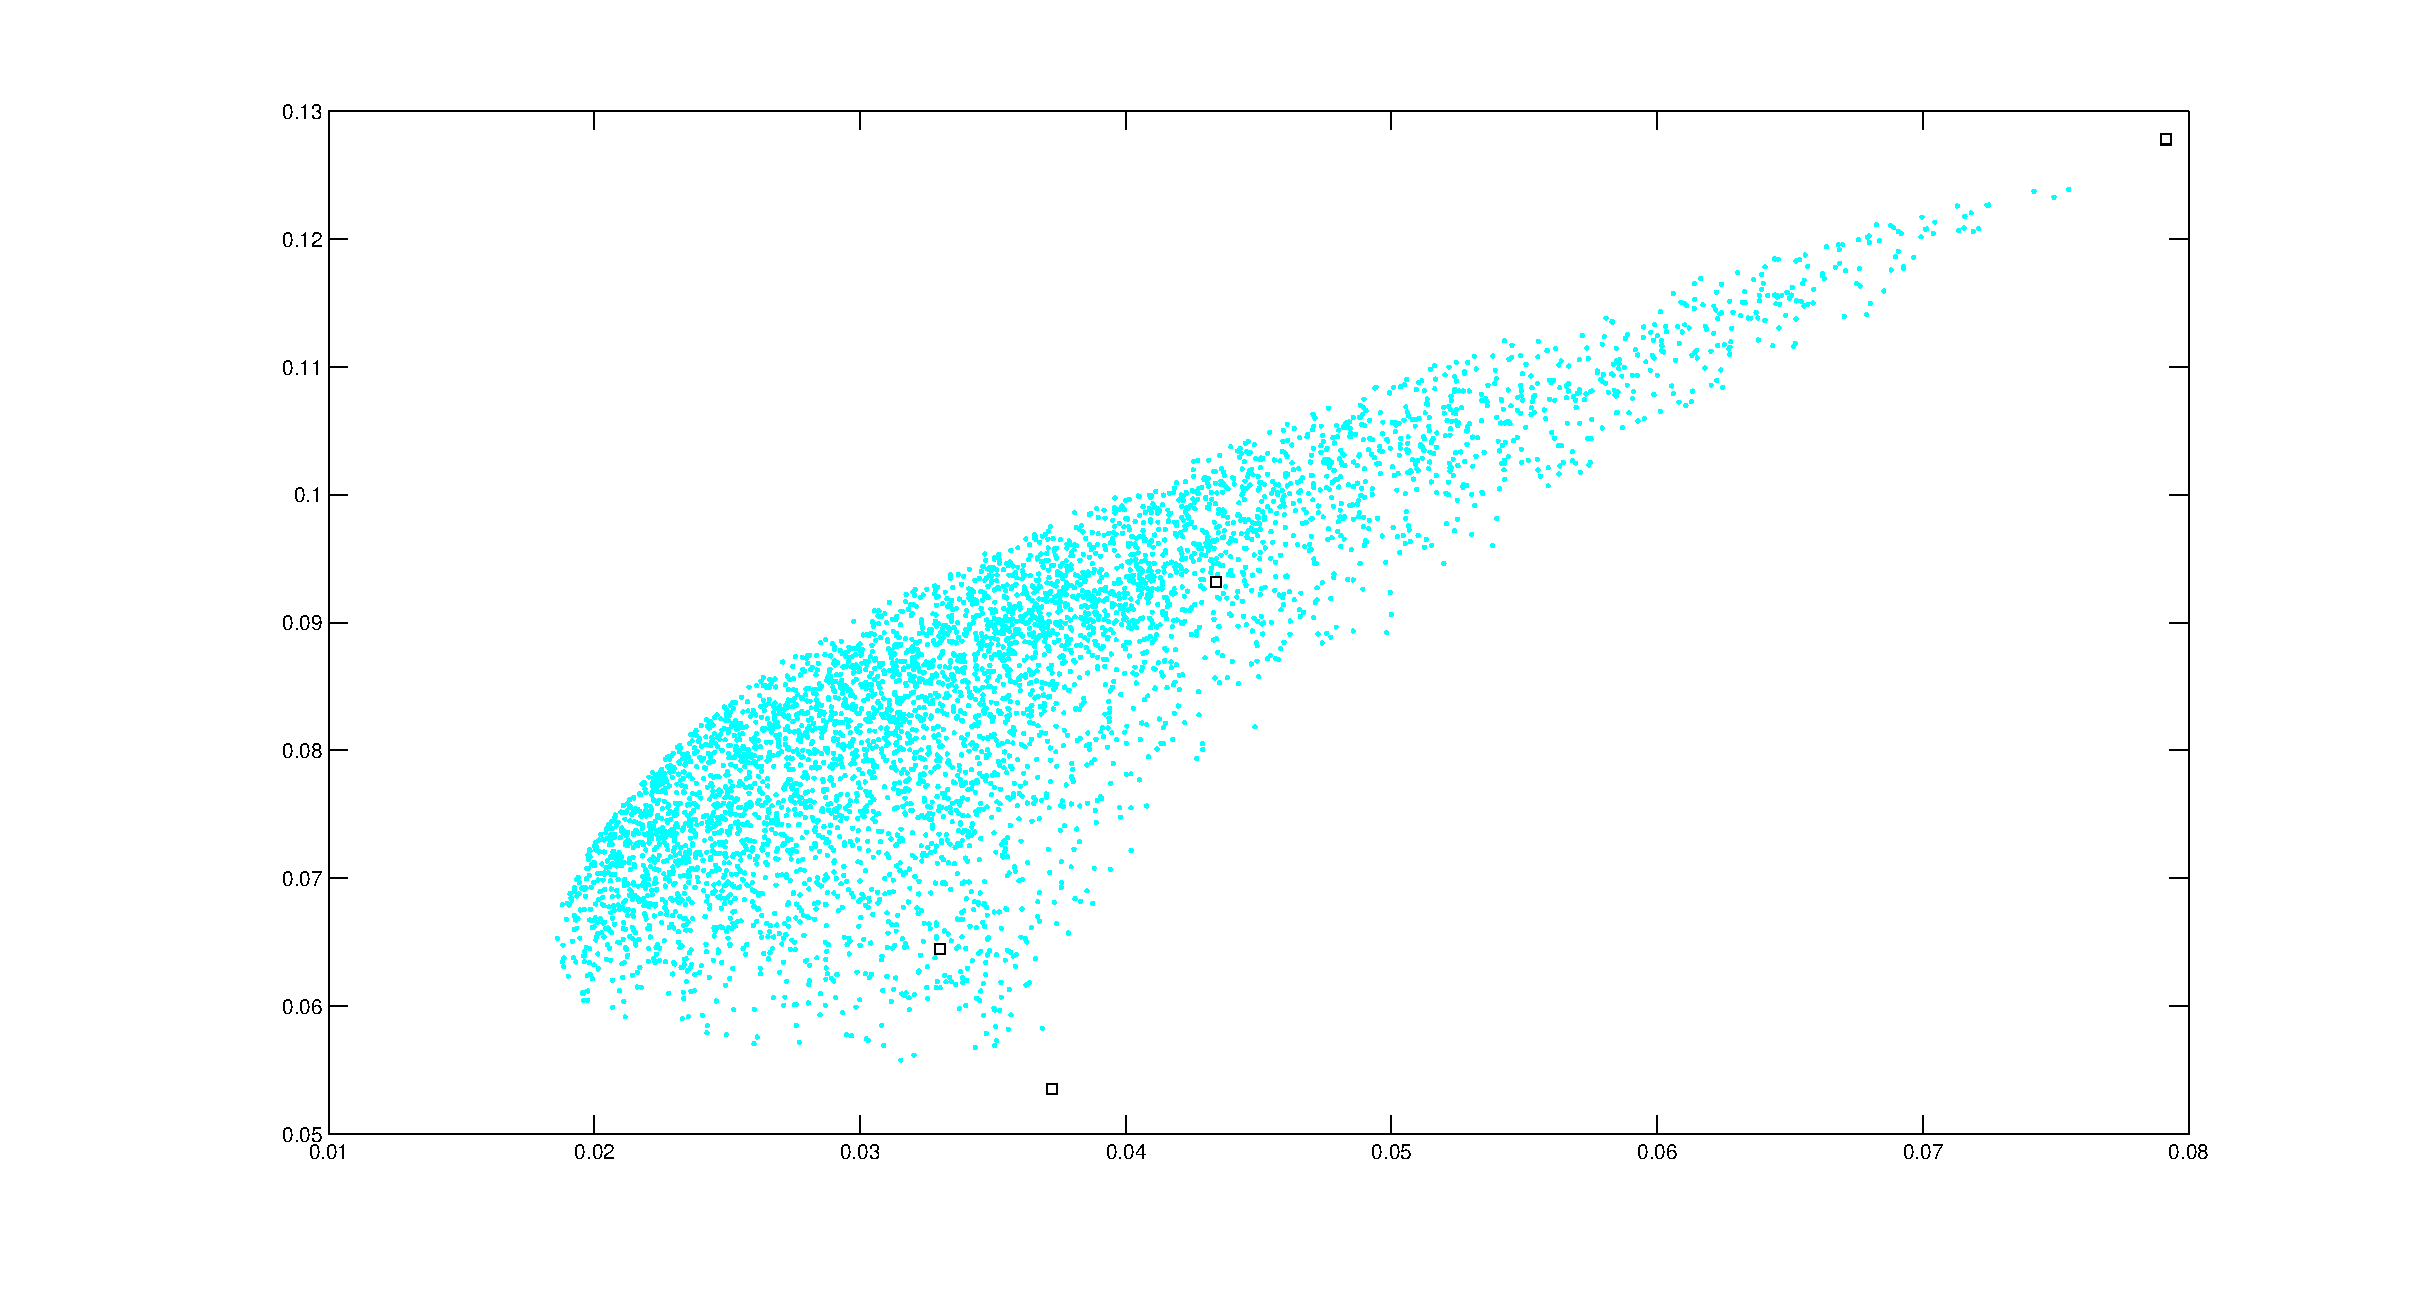
\includegraphics[scale = .39]{ExercisePOS.eps}
		\caption{Based on this graph, we can see that security \textit{d} is the dominated security.}
	\end{center}
\end{figure}

\subsection{The Efficient Frontier}

\begin{verbatim}
  frontcon(ExpReturns, Covariance, 500)
\end{verbatim}
generates the graph of the efficient frontier shown below.
\begin{figure}[h]
	\begin{center}
		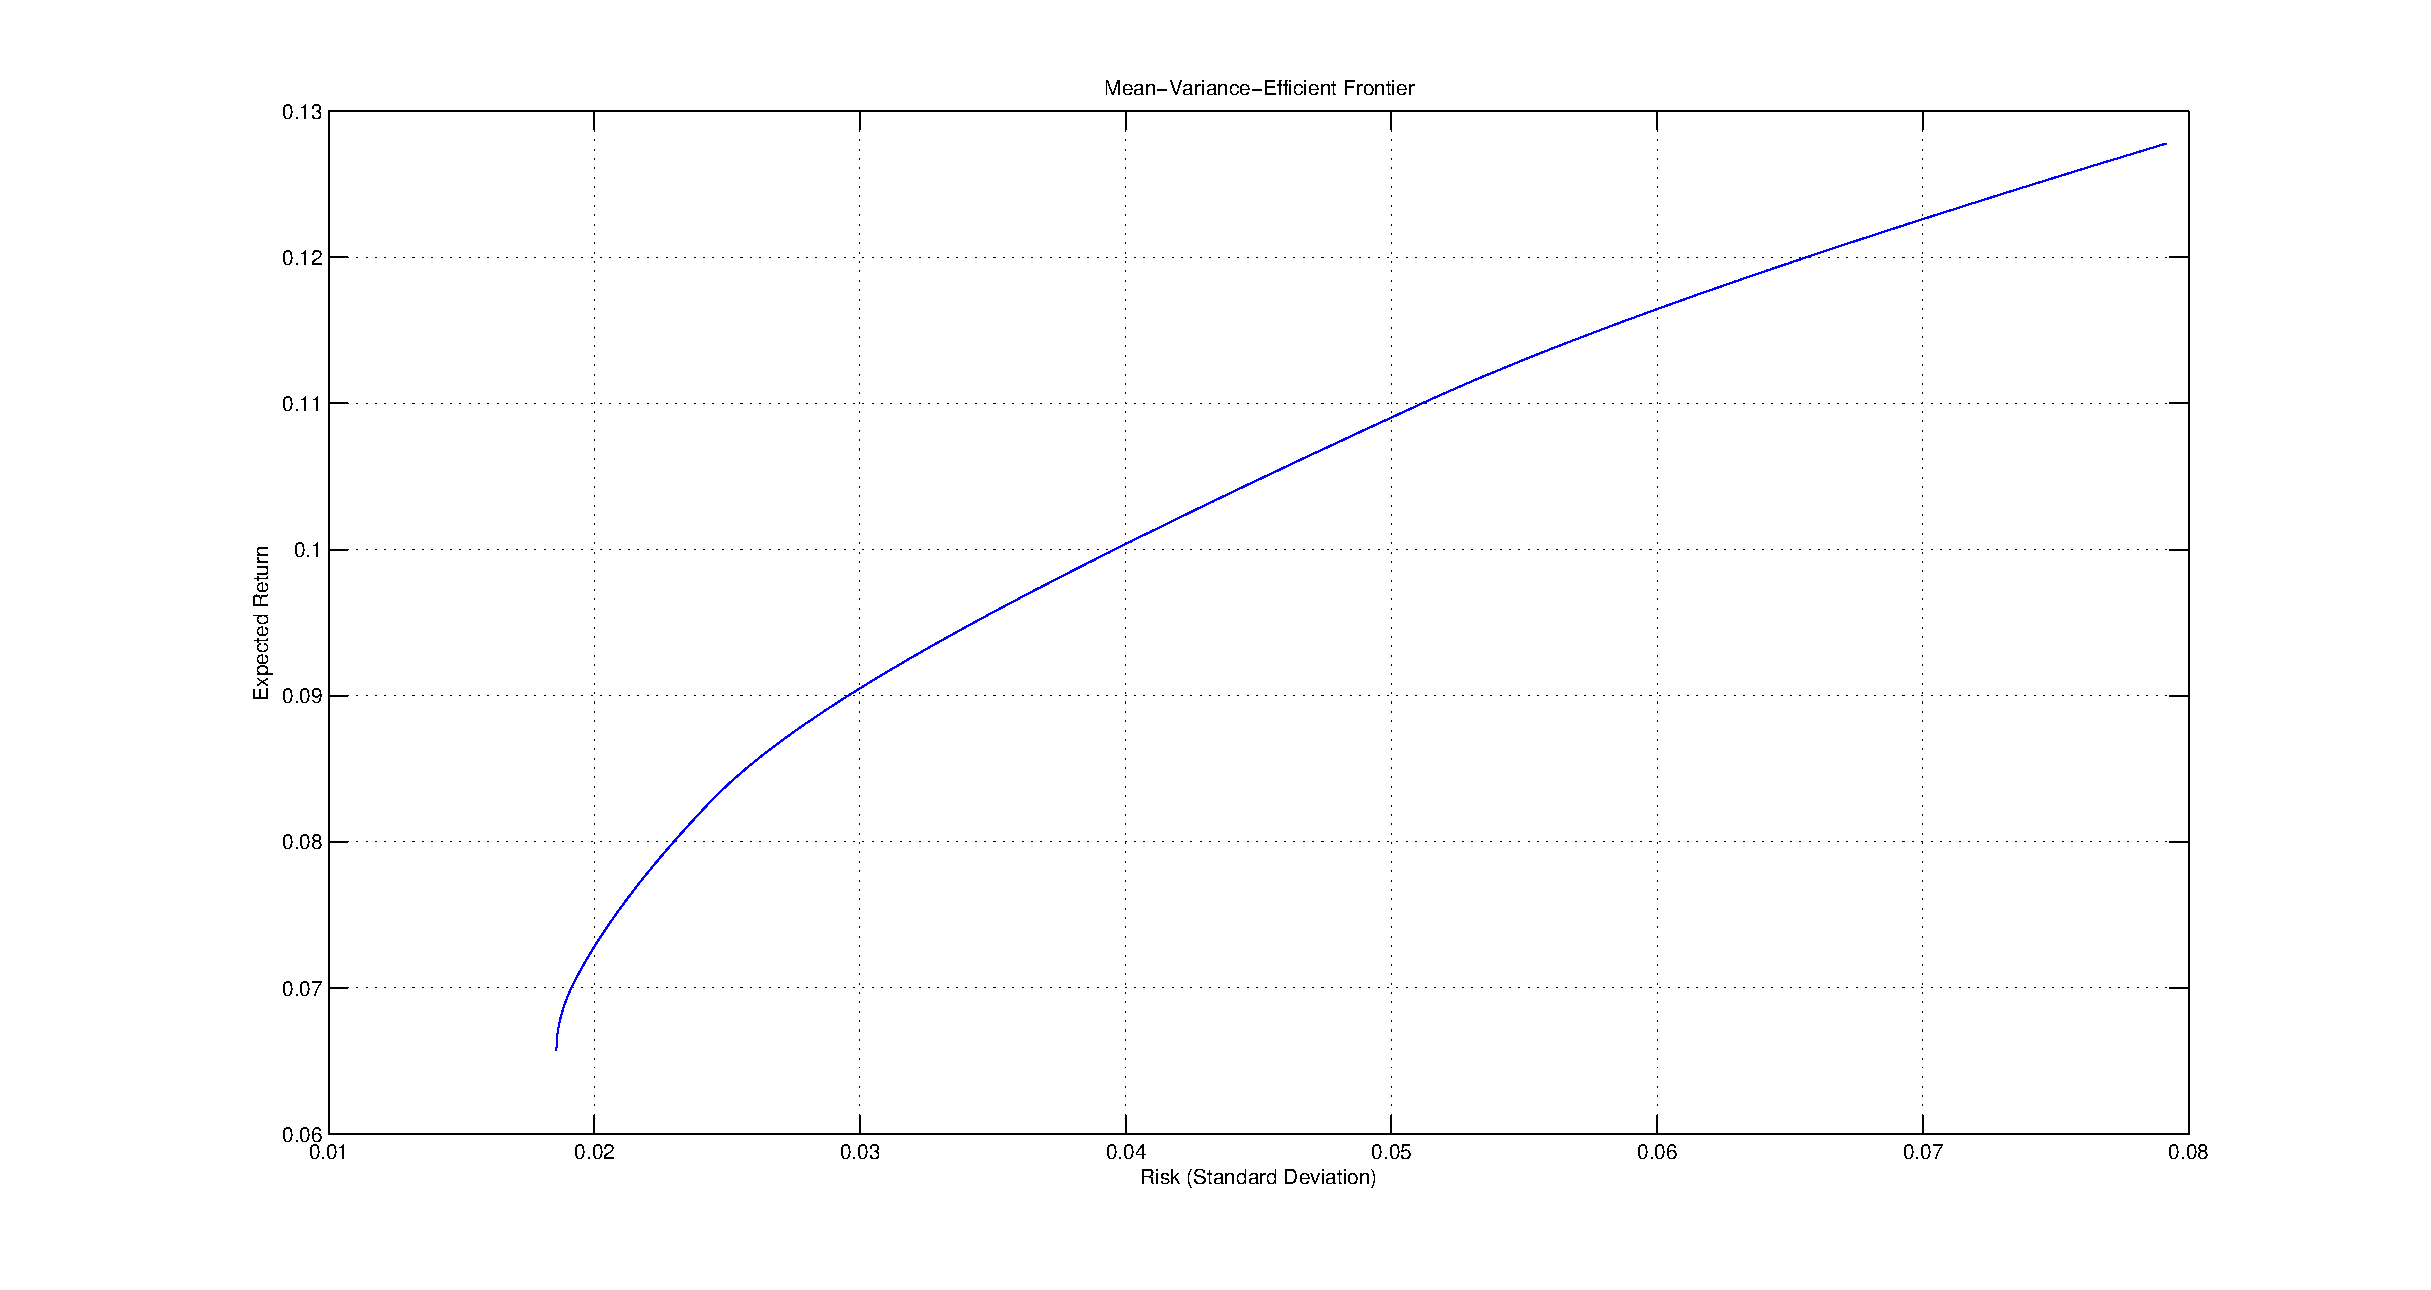
\includegraphics[scale = .37]{ExerciseEffFront.eps}
	\end{center}
\end{figure}

\subsection{Risk Aversion}
Using our functions \texttt{buildFIS} and \texttt{evaluateFIS}:
\begin{verbatim}
  fis = buildFIS()
  evaluateFIS(45, 20, fis)
  evaluateFIS(50, 65, fis)
\end{verbatim}
which outputs:
\begin{verbatim}
  ans =
    3.7305
  ans =
    8.3077
\end{verbatim}

\subsection{Constructing the Complete Optimal Portfolio}
\begin{verbatim}
  [PortRisk, PortReturn, PortWts] = frontcon(ExpReturns, Covariance);
  [RiskyRisk, RiskyReturn, RiskyWts, RiskyFraction, OverallRisk, OverallReturn] = ...
    portalloc(PortRisk, PortReturn, PortWts, .02, NaN, 8.3077);
  fprintf(`The composition of the complete portfolios is:\n\ta = %5.3f%%\n
    ...\tb = %5.3f%%\n\tc = %5.3f%%\n\td = %5.3f%%\n\trisk-free = %5.3f%%\n', ...
   RiskyFraction*RiskyWts(1)*100, RiskyFraction*RiskyWts(2)*100, 
   ...RiskyFraction*RiskyWts(3)*100, RiskyFraction*RiskyWts(4)*100,...
   (1 - RiskyFraction)*100)
  fprintf(`The expected return of the complete portfolio is %5.3f%%\n',...
    OverallReturn*100)
  fprintf(`The standard deviation of the complete portfolio is %5.3f%%\n',...
    OverallRisk*100)
\end{verbatim}
which will output the following:
\begin{verbatim}
  The composition of the complete portfolios is:
    a = 84.798%
    b = 15.202%
    c = 0.000%
    d = 0.000%
    risk-free = 0.000%
  The expected return of the complete portfolio is 12.251%
  The standard deviation of the complete portfolio is 6.986%
\end{verbatim}
Notice that in this example, the investor puts 100\% of his available capital into the risky portfolio.

\section{References}
\begin{itemize}
	\item{Bodie, Kane, and Marcus, \textit{Investments}, $8^{th}$ Edition, McGraw-Hill, Chapters 6 \& 7.}
	\item{French, Kenneth R. Tuck School of Business. Darthmouth University. Web. 09 May 2011. $<$http://mba.tuck.dartmouth.edu/pages/faculty/ken.french/$>$.}
	\item{MathWorks, MATLAB R2010a Product Documentation, Financial Toolbox.}
\end{itemize}

\end{document} 